\documentclass[12pt,a4paper,twoside,openright,titlepage,final]{article}
\usepackage{fontspec}
\usepackage{amsmath}
\usepackage{amsfonts}
\usepackage{amssymb}
\usepackage{makeidx}
\usepackage{graphicx}
\usepackage[hidelinks,unicode=true]{hyperref}
\usepackage[spanish,es-nodecimaldot,es-lcroman,es-tabla,es-noshorthands]{babel}
\usepackage[left=3cm,right=2cm, bottom=4cm]{geometry}
\usepackage{natbib}
\usepackage{microtype}
\usepackage{ifdraft}
\usepackage{verbatim}
\usepackage[nottoc]{tocbibind}
\usepackage{pdflscape}
\usepackage[obeyDraft]{todonotes}
\ifdraft{
	\usepackage{draftwatermark}
	\SetWatermarkText{BORRADOR}
	\SetWatermarkScale{0.7}
	\SetWatermarkColor{red}
}{}
\usepackage{booktabs}
\usepackage{longtable}
\usepackage{calc}
\usepackage{array}
\usepackage{caption}
\usepackage{subfigure}
\usepackage{footnote}
\usepackage{url}
\usepackage[titletoc]{appendix}

\setsansfont[Ligatures=TeX]{texgyreadventor}
\setmainfont[Ligatures=TeX]{texgyrepagella}
\setmonofont{FreeMono}

\usetikzlibrary{decorations.pathreplacing}

%*******************************************************
%                 NO MODIFICAR
\newcommand*{\FSfont}[1]{%
  \fontencoding{T1}\fontfamily{#1}\selectfont}

\newlength{\tpheight}\setlength{\tpheight}{0.9\textheight}
\newlength{\txtheight}\setlength{\txtheight}{0.9\tpheight}
\newlength{\tpwidth}\setlength{\tpwidth}{0.9\textwidth}
\newlength{\txtwidth}\setlength{\txtwidth}{0.9\tpwidth}
\newlength{\drop}
%*******************************************************

% Crea una portada con los siguientes parámetros
%
% #1 : Título 
% #2 : Subtítulo
% #3 : Subsubtítulo
% #4 : Autor(es)
% #5 : Lugar
%

\newcommand*{\portada}[5]{
\begin{titlepage}
\begingroup
\vspace*{1cm}
\drop = 0.2\txtheight
\centering
\vfill
{\Huge \scshape #1}\\[\baselineskip]
{\Large \textbf{#2}}\\[\baselineskip]
{\Large \scshape #3}\\[\baselineskip]
\vspace*{0.3cm}
{\large \textit{#4}}\\[0.5\drop]

\includegraphics[scale=0.35]{./imagenes/logoURJC.jpg}
\vspace*{1.5cm}

{\large \scshape #5, \today} \par
\begin{center}
\end{center}
\vfill\null
\endgroup
\end{titlepage}
}
 %*****************************************************
 


\author{José Ignacio Escribano}

\title{}

\setlength{\parindent}{0pt}

\begin{document}

\pagenumbering{alph}
\setcounter{page}{1}

\portada{Caso Práctico IV}{Minería de datos}{Árboles y reglas de de decisión}{José Ignacio Escribano}{Móstoles}

\listoffigures
\thispagestyle{empty}
\newpage

\tableofcontents
\thispagestyle{empty}
\newpage


\pagenumbering{arabic}
\setcounter{page}{1}

\section{Introducción}

En este caso práctico utilizaremos los árboles como herramienta de clasificación. Utilizaremos dos bases de datos conocidas \texttt{iris} y \texttt{spam7}. La primera, muestra tres tipos de especies de iris a partir de distintas medidas de los pétalos y sépalos. La segunda, clasifica el spam a partir de distintas palabras o símbolos que se encuentran en los correos electrónicos.

\section{Resolución de las cuestiones de evaluación}

A continuación, resolvemos las cuestiones de evaluación planteadas.

\subsection{Cuestión 1}

En esta primera cuestión, utilizaremos la base de datos \texttt{iris}, que clasifica tres especies de iris de acuerdo a cuatro variables: longitud y anchura del sépalo, y longitud y anchura del pétalo.\\

Comenzamos representando el árbol de decisión para estos datos (Figura~\ref{fig:iris_sin_podar}).\\

\begin{figure}[tbph!]
\centering
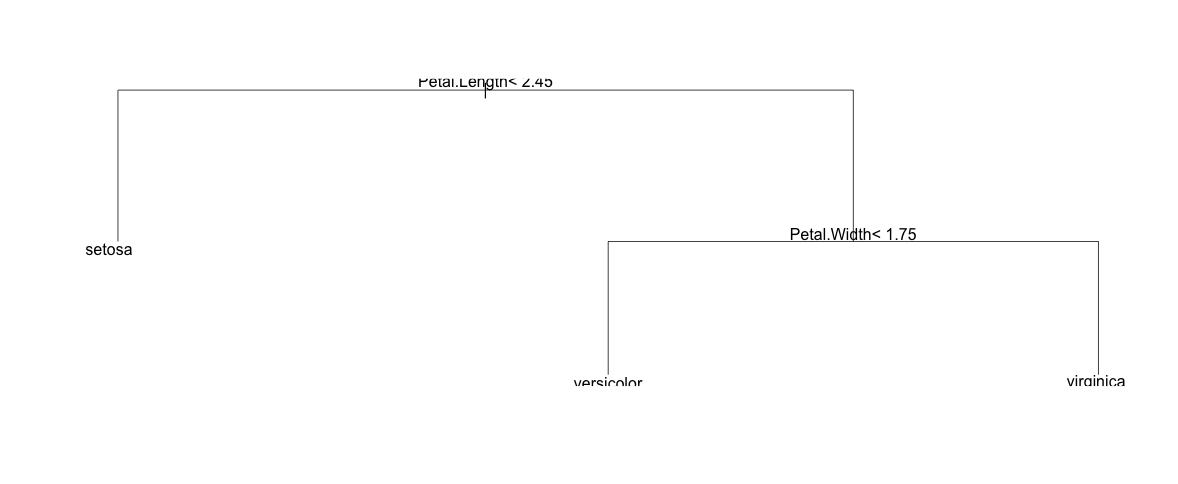
\includegraphics[width=0.9\linewidth]{imagenes/iris_sin_podar}
\caption{Árbol de decisión de la base de datos iris}
\label{fig:iris_sin_podar}
\end{figure}

Vemos que este árbol clasifica la especie setosa si la longitud del pétalo es menor que 2.45. Para las demás especies tiene en cuenta la anchura del pétalo: si es menor que 1.75 tendremos la especie versicolor, en caso contrario, la especie virginica.\\

Procedemos a podar este árbol. Para ello, representamos el gráfico donde se representa el número de nodos del árbol, el error cometido y la complejidad del árbol (Figura~\ref{fig:cp_plot}).\\

\begin{figure}[tbph!]
\centering
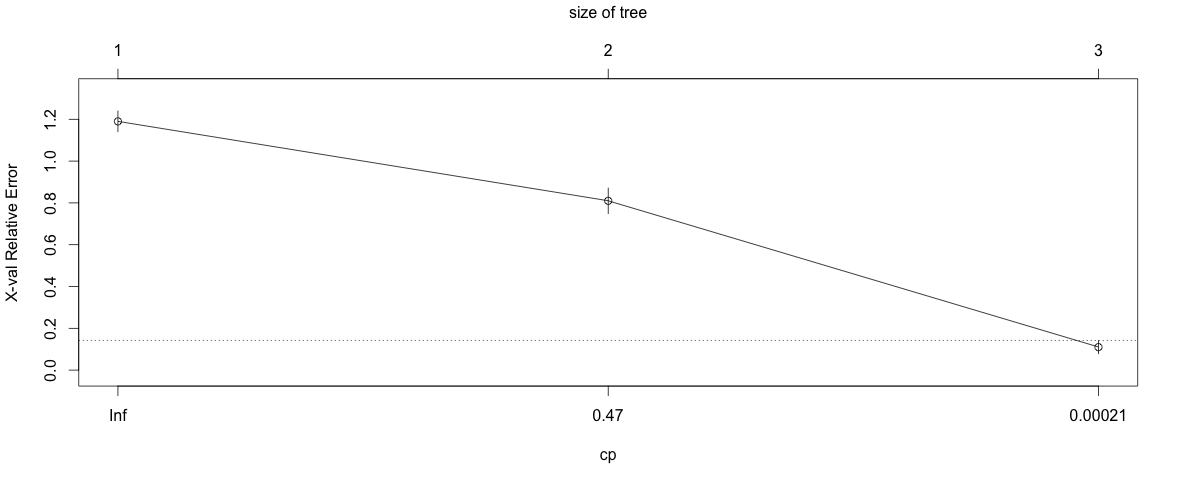
\includegraphics[width=0.8\linewidth]{imagenes/cp_plot}
\caption{Error y complejidad del árbol de decisión antes de podar}
\label{fig:cp_plot}
\end{figure}

Observamos que el error más pequeño se comete cuando el número de nodos del árbol es 3. Calculamos, usando R, el valor óptimo de este valor. Se tiene que el valor pedido es $10^{-7}$. Con este valor ya estamos en disposición de podar el árbol (Figura~\ref{fig:iris_arbol_podado}).\\

\begin{figure}[tbph!]
\centering
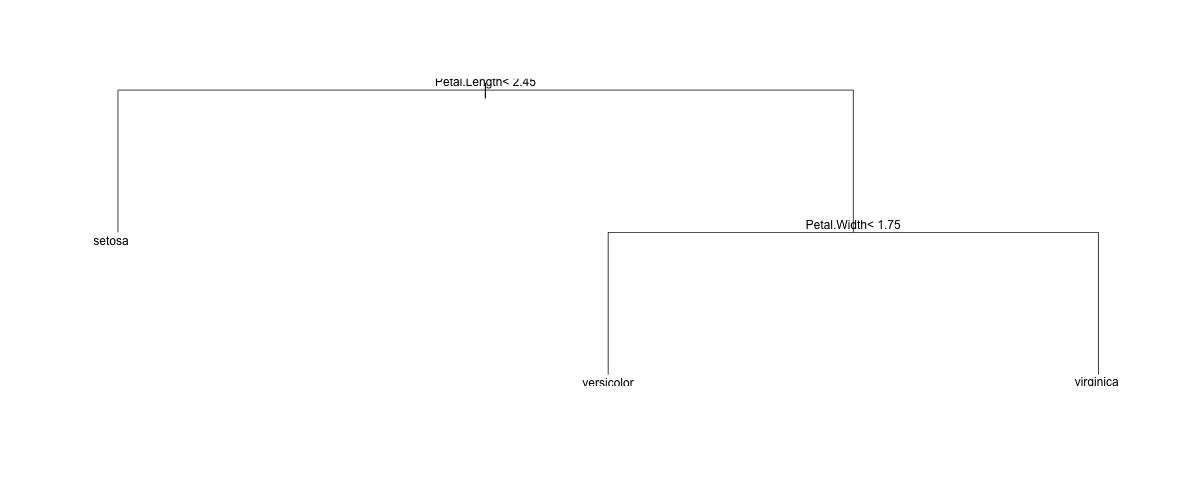
\includegraphics[width=0.9\linewidth]{imagenes/iris_arbol_podado}
\caption{Árbol de decisión podado de la base de datos iris}
\label{fig:iris_arbol_podado}
\end{figure}

Vemos que es el árbol podado es el mismo que sin podar, por lo que en este caso, podar no consigue un árbol más pequeño que el árbol inicial. Esta técnica de podado puede ser útil cuando el árbol tiene muchos nodos y ramas, y se quiere eliminar alguna para que sea más comprensible y además, evitar el sobreajuste. 

\subsection{Cuestión 2}

En esta cuestión utilizaremos la base de datos \texttt{spam7} disponible en el paquete de DAAG de R. Esta base de datos consta de seis variables explicativas para medir la presencia de spam en emails: crl.tot (longitud de las palabras que están en mayúsculas), dollar (frecuencia del símbolo ``\$'' en términos del porcentaje respecto de caracteres), bang (frecuencia del símbolo ``!'' en términos del porcentaje respecto de caracteres), money (frecuencia de la palabra ``money'' en términos del porcentaje respecto de caracteres), n000 (frecuencia de la cadena ``n000'' en términos del porcentaje respecto de caracteres) y make (frecuencia de la palabra ``make'' en términos del porcentaje respecto de caracteres).\\

Calculamos el árbol de decisión usando el paquete tree de R. Un resumen del árbol se puede ver a continuación:

\begin{verbatim}
Classification tree:
tree(formula = yesno ~ ., data = spam7)
Variables actually used in tree construction:
[1] "dollar"  "bang"    "crl.tot" "money"  
Number of terminal nodes:  8 
Residual mean deviance:  0.7116 = 3268 / 4593 
Misclassification error rate: 0.1445 = 665 / 4601 
\end{verbatim}

Vemos que este el árbol tiene 8 nodos terminales, con un error del 14.45\%, o lo que es lo mismo, clasifica de forma incorrecta 665 de los 4601 emails. La estructura del árbol es la siguiente:

\begin{verbatim}
node), split, n, deviance, yval, (yprob)
      * denotes terminal node

 1) root 4601 6170.00 n ( 0.60596 0.39404 )  
   2) dollar < 0.0555 3471 3786.00 n ( 0.76491 0.23509 )  
     4) bang < 0.0875 2407 1571.00 n ( 0.89946 0.10054 ) *
     5) bang > 0.0875 1064 1468.00 y ( 0.46053 0.53947 )  
      10) crl.tot < 85.5 541  681.10 n ( 0.67652 0.32348 ) *
      11) crl.tot > 85.5 523  572.90 y ( 0.23709 0.76291 )  
        22) bang < 0.5155 342  440.70 y ( 0.34503 0.65497 )  
          44) money < 0.04 262  360.20 y ( 0.44656 0.55344 ) *
          45) money > 0.04 80   10.75 y ( 0.01250 0.98750 ) *
        23) bang > 0.5155 181   52.68 y ( 0.03315 0.96685 ) *
   3) dollar > 0.0555 1130  818.80 y ( 0.11770 0.88230 )  
     6) bang < 0.0775 275  355.80 y ( 0.34909 0.65091 )  
      12) money < 0.025 167  231.00 n ( 0.52695 0.47305 ) *
      13) money > 0.025 108   57.04 y ( 0.07407 0.92593 ) *
     7) bang > 0.0775 855  304.70 y ( 0.04327 0.95673 ) *
\end{verbatim}

El árbol utiliza las variables dollar, bang, crl.tot y money. El árbol se puede ver en la Figura~\ref{fig:spam_plot}.\\

\begin{figure}[tbph!]
\centering
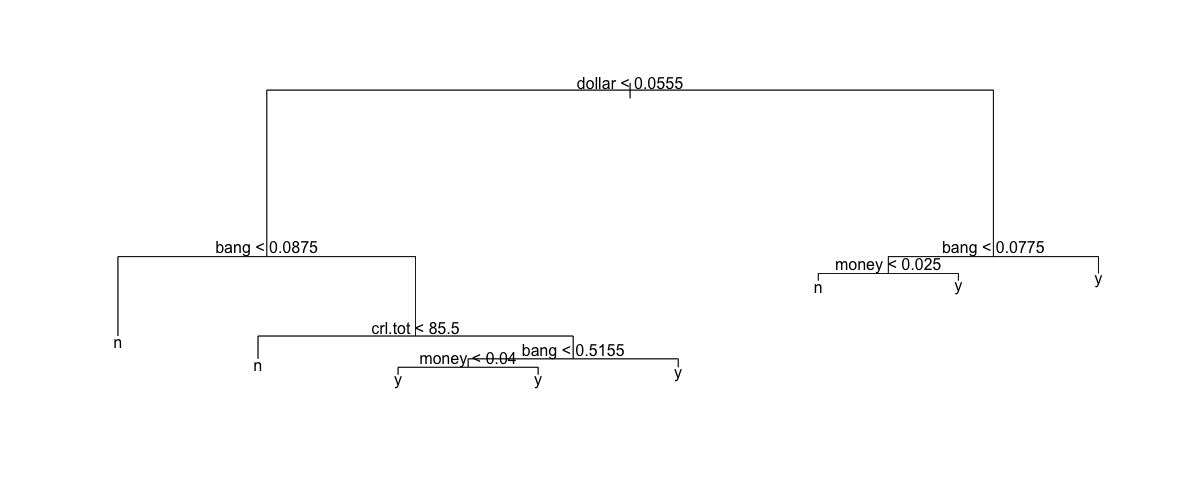
\includegraphics[width=0.9\linewidth]{imagenes/spam_plot}
\caption{Árbol de decisión de la base de datos spam7}
\label{fig:spam_plot}
\end{figure}

De acuerdo al árbol de la Figura~\ref{fig:spam_plot}, se pueden establecer las reglas de decisión para establecer si un correo es o no spam. Los casos de spam y no spam son respectivamente los siguientes:

\begin{itemize}
	\item Spam
	
	\begin{enumerate}
		\item $\text{dollar} < 0.0555$ y $\text{dollar} \geq 0.0875$ y $\text{crl.tot} \geq 85.5$ y $\text{bang} \geq 0.5155$
		
		\item $\text{dollar} < 0.0555$ y $\text{dollar} \geq 0.0875$ y $\text{crl.tot} \geq 85.5$ y $\text{money}$\footnote{Notar que los hijos del nodo money conducen a la presencia de spam, independientemente de la frecuencia de esta palabra en el email.}
		
		\item $\text{dollar} \geq 0.0555$ y $\text{bang} \geq 0.0775$
		
		\item $\text{dollar} \geq 0.0555$ y $\text{bang} < 0.0775$ y $\text{money} \geq 0.025$
	\end{enumerate}
	
	\item No spam
	
	\begin{enumerate}
		\item $\text{dollar} < 0.0555$ y $\text{bang} < 0.0875$
		
		\item $\text{dollar} < 0.0555$ y $\text{bang} \geq 0.0875$ y $\text{crt.tot} < 85.5$
		
		\item $\text{dollar} \geq 0.0555$ y $\text{bang} < 0.0775$ y $\text{money} < 0.025$
		
	\end{enumerate}
\end{itemize}

\section{Conclusiones}

En este caso práctico hemos visto cómo crear árboles de decisión y podarlos, si fuera necesario. Los árboles de decisión son una técnica de minería de datos muy potente, ya que es fácilmente entendible por las personas, y muy fácil de programar el modelo obtenido.\\

R nos ha permitido ahorrar mucho tiempo debido a las librerías que implementan árboles. Existen diferentes librerías que implementan los árboles de decisión, por lo que antes de utilizar una u otra será necesario conocer la documentación y los algoritmos que implementa cada una de ellas, de acuerdo al problema que estemos tratando. 

\clearpage

\section{Código R utilizado}

\verbatiminput{caso_4.R}

\end{document}